% Options for packages loaded elsewhere
\PassOptionsToPackage{unicode}{hyperref}
\PassOptionsToPackage{hyphens}{url}
%
\documentclass[
  12pt,
  ignorenonframetext,
  aspectratio=169,
]{beamer}
\usepackage{pgfpages}
\setbeamertemplate{caption}[numbered]
\setbeamertemplate{caption label separator}{: }
\setbeamercolor{caption name}{fg=normal text.fg}
\beamertemplatenavigationsymbolsempty
% Prevent slide breaks in the middle of a paragraph
\widowpenalties 1 10000
\raggedbottom

\usepackage{amsmath,amssymb}
\usepackage{iftex}
\ifPDFTeX
  \usepackage[T1]{fontenc}
  \usepackage[utf8]{inputenc}
  \usepackage{textcomp} % provide euro and other symbols
\else % if luatex or xetex
  \usepackage{unicode-math}
  \defaultfontfeatures{Scale=MatchLowercase}
  \defaultfontfeatures[\rmfamily]{Ligatures=TeX,Scale=1}
\fi
\usepackage{lmodern}
\ifPDFTeX\else  
    % xetex/luatex font selection
\fi
% Use upquote if available, for straight quotes in verbatim environments
\IfFileExists{upquote.sty}{\usepackage{upquote}}{}
\IfFileExists{microtype.sty}{% use microtype if available
  \usepackage[]{microtype}
  \UseMicrotypeSet[protrusion]{basicmath} % disable protrusion for tt fonts
}{}
\makeatletter
\@ifundefined{KOMAClassName}{% if non-KOMA class
  \IfFileExists{parskip.sty}{%
    \usepackage{parskip}
  }{% else
    \setlength{\parindent}{0pt}
    \setlength{\parskip}{6pt plus 2pt minus 1pt}}
}{% if KOMA class
  \KOMAoptions{parskip=half}}
\makeatother
\usepackage{xcolor}
\newif\ifbibliography
\setlength{\emergencystretch}{3em} % prevent overfull lines
\setcounter{secnumdepth}{-\maxdimen} % remove section numbering


\providecommand{\tightlist}{%
  \setlength{\itemsep}{0pt}\setlength{\parskip}{0pt}}\usepackage{longtable,booktabs,array}
\usepackage{calc} % for calculating minipage widths
\usepackage{caption}
% Make caption package work with longtable
\makeatletter
\def\fnum@table{\tablename~\thetable}
\makeatother
\usepackage{graphicx}
\makeatletter
\def\maxwidth{\ifdim\Gin@nat@width>\linewidth\linewidth\else\Gin@nat@width\fi}
\def\maxheight{\ifdim\Gin@nat@height>\textheight\textheight\else\Gin@nat@height\fi}
\makeatother
% Scale images if necessary, so that they will not overflow the page
% margins by default, and it is still possible to overwrite the defaults
% using explicit options in \includegraphics[width, height, ...]{}
\setkeys{Gin}{width=\maxwidth,height=\maxheight,keepaspectratio}
% Set default figure placement to htbp
\makeatletter
\def\fps@figure{htbp}
\makeatother

\usepackage{booktabs}
\usepackage{longtable}
\usepackage{array}
\usepackage{multirow}
\usepackage{wrapfig}
\usepackage{float}
\usepackage{colortbl}
\usepackage{pdflscape}
\usepackage{tabu}
\usepackage{threeparttable}
\usepackage{threeparttablex}
\usepackage[normalem]{ulem}
\usepackage{makecell}
\usepackage{xcolor}
\makeatletter
\@ifpackageloaded{tcolorbox}{}{\usepackage[skins,breakable]{tcolorbox}}
\@ifpackageloaded{fontawesome5}{}{\usepackage{fontawesome5}}
\definecolor{quarto-callout-color}{HTML}{909090}
\definecolor{quarto-callout-note-color}{HTML}{0758E5}
\definecolor{quarto-callout-important-color}{HTML}{CC1914}
\definecolor{quarto-callout-warning-color}{HTML}{EB9113}
\definecolor{quarto-callout-tip-color}{HTML}{00A047}
\definecolor{quarto-callout-caution-color}{HTML}{FC5300}
\definecolor{quarto-callout-color-frame}{HTML}{acacac}
\definecolor{quarto-callout-note-color-frame}{HTML}{4582ec}
\definecolor{quarto-callout-important-color-frame}{HTML}{d9534f}
\definecolor{quarto-callout-warning-color-frame}{HTML}{f0ad4e}
\definecolor{quarto-callout-tip-color-frame}{HTML}{02b875}
\definecolor{quarto-callout-caution-color-frame}{HTML}{fd7e14}
\makeatother
\makeatletter
\@ifpackageloaded{caption}{}{\usepackage{caption}}
\AtBeginDocument{%
\ifdefined\contentsname
  \renewcommand*\contentsname{Table of contents}
\else
  \newcommand\contentsname{Table of contents}
\fi
\ifdefined\listfigurename
  \renewcommand*\listfigurename{List of Figures}
\else
  \newcommand\listfigurename{List of Figures}
\fi
\ifdefined\listtablename
  \renewcommand*\listtablename{List of Tables}
\else
  \newcommand\listtablename{List of Tables}
\fi
\ifdefined\figurename
  \renewcommand*\figurename{Figure}
\else
  \newcommand\figurename{Figure}
\fi
\ifdefined\tablename
  \renewcommand*\tablename{Table}
\else
  \newcommand\tablename{Table}
\fi
}
\@ifpackageloaded{float}{}{\usepackage{float}}
\floatstyle{ruled}
\@ifundefined{c@chapter}{\newfloat{codelisting}{h}{lop}}{\newfloat{codelisting}{h}{lop}[chapter]}
\floatname{codelisting}{Listing}
\newcommand*\listoflistings{\listof{codelisting}{List of Listings}}
\makeatother
\makeatletter
\makeatother
\makeatletter
\@ifpackageloaded{caption}{}{\usepackage{caption}}
\@ifpackageloaded{subcaption}{}{\usepackage{subcaption}}
\makeatother

\ifLuaTeX
  \usepackage{selnolig}  % disable illegal ligatures
\fi
\usepackage{bookmark}

\IfFileExists{xurl.sty}{\usepackage{xurl}}{} % add URL line breaks if available
\urlstyle{same} % disable monospaced font for URLs
\hypersetup{
  pdftitle={Uncertainty Estimation for High-dimensional Nonparametric Forecasting},
  pdfauthor={Nuwani Palihawadana},
  hidelinks,
  pdfcreator={LaTeX via pandoc}}

\usetheme{Monash}


% Monash title page
% Modified by moving title and adding collaborators
\setbeamerfont{title}{series=\bfseries,parent=structure,size=\fontsize{20}{28}}
\setbeamertemplate{title page}
{\placefig{-0.01}{-0.01}{width=1.01\paperwidth,height=1.01\paperheight}{bg-13.png}
\begin{textblock}{10.2}(1,1)\usebeamerfont{title}
{\color{white}\raggedright\par\inserttitle}
\end{textblock}
\begin{textblock}{8.7}(1,5.3)
{\color{white}\raggedright{\insertauthor}\mbox{}\\[0.2cm]}
\end{textblock}
\begin{textblock}{10.8}(1,6.6)
{\color{white}\raggedright{\textbf{Joint work with :} Rob Hyndman, Xiaoqian Wang}\mbox{}\\[0.2cm]
\insertdate}
\end{textblock}}


% Find images
\graphicspath{{_extensions/presentation/_images/background/}{_extensions/quarto-monash/presentation/_images/background/}{figs/}{figures/}{images/}{img/}}
\title{Uncertainty Estimation for High-dimensional Nonparametric
Forecasting}
\author{Nuwani Palihawadana}
\date{1 July 2025}
\titlegraphic{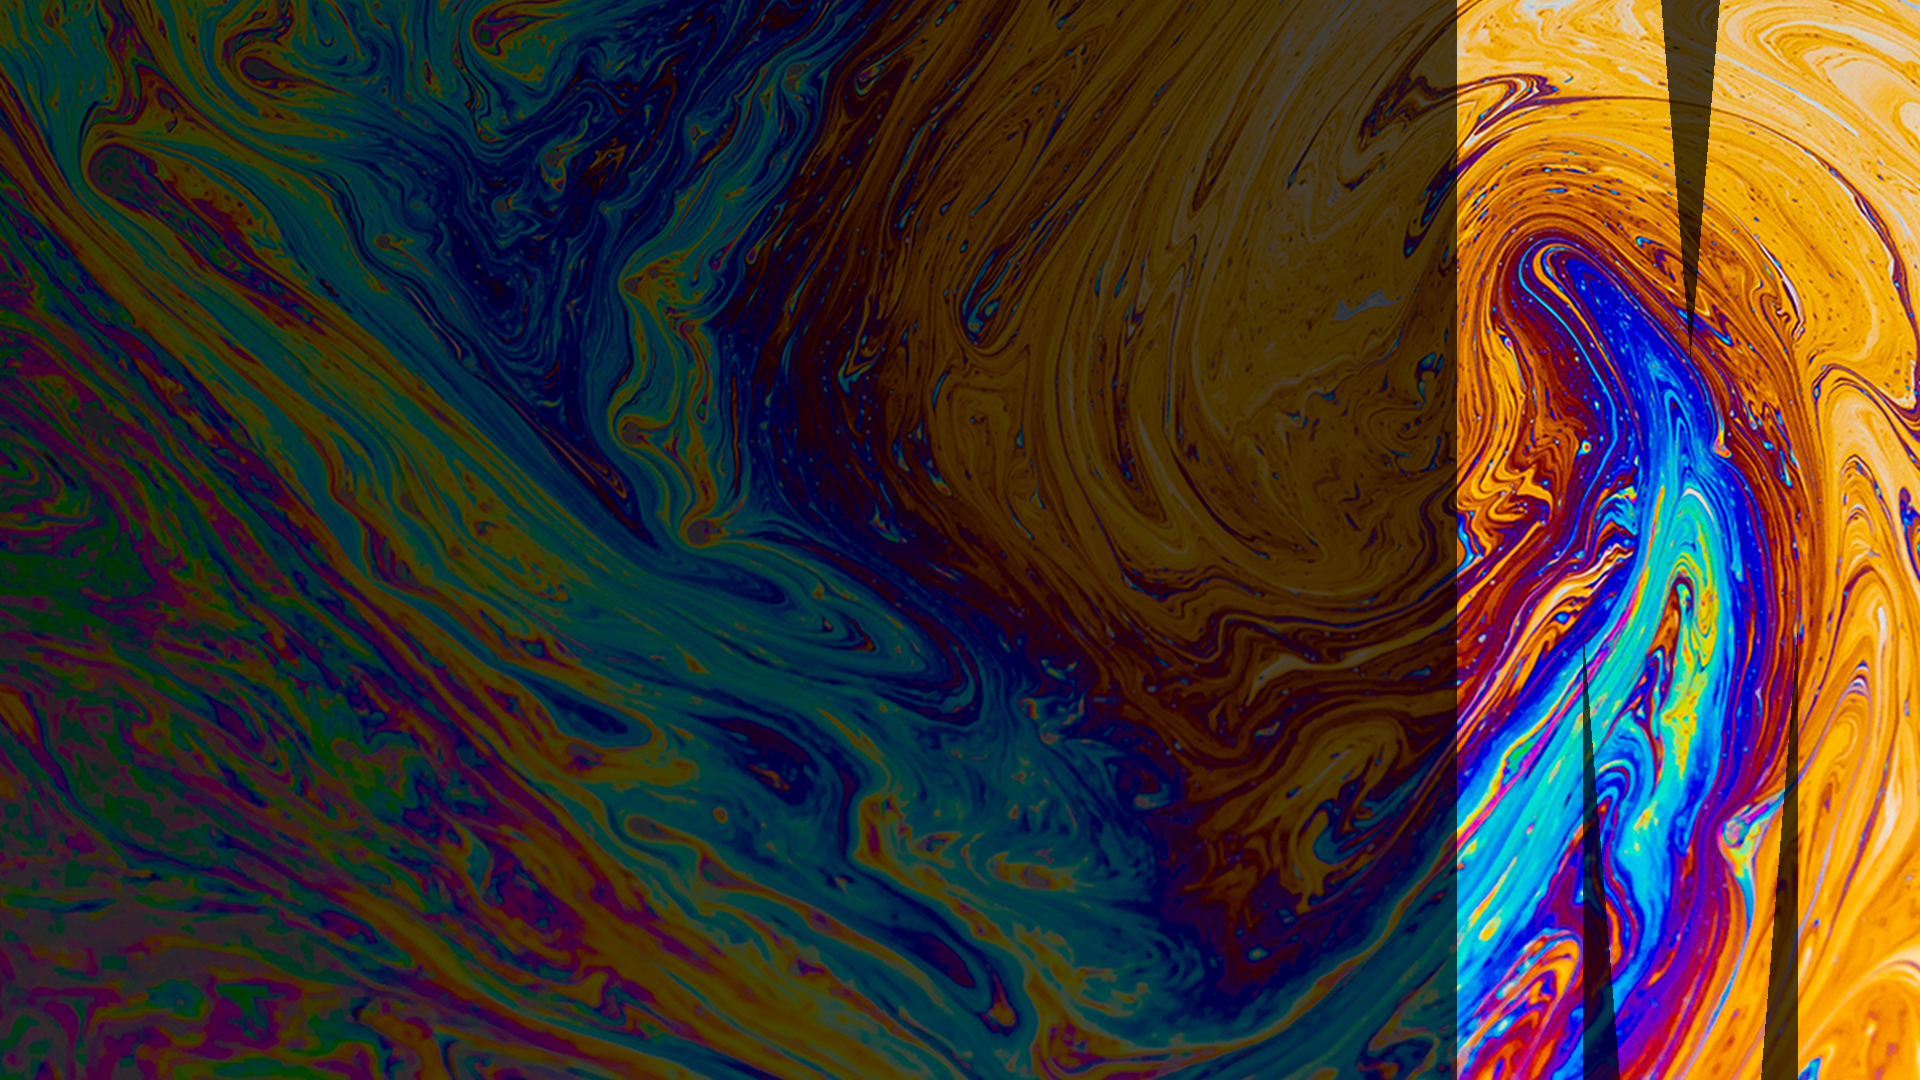
\includegraphics{bg-13.png}}

\begin{document}
\frame{\titlepage}


\begin{frame}{Nonparametric forecasting}
\phantomsection\label{nonparametric-forecasting}
\placefig{0.5}{1.4}{width=15cm}{nonpara1}
\end{frame}

\begin{frame}{Nonparametric forecasting}
\phantomsection\label{nonparametric-forecasting-1}
\placefig{0.5}{1.3}{width=15cm}{nonpara2}
\end{frame}

\begin{frame}{Sparse Multiple Index (SMI) model}
\phantomsection\label{sparse-multiple-index-smi-model}
\placefig{0.5}{1.5}{width=15cm}{smi1}
\end{frame}

\begin{frame}{Sparse Multiple Index (SMI) model}
\phantomsection\label{sparse-multiple-index-smi-model-1}
\placefig{0.5}{1.5}{width=15cm}{smi2}
\end{frame}

\begin{frame}{Sparse Multiple Index (SMI) model}
\phantomsection\label{sparse-multiple-index-smi-model-2}
\placefig{0.5}{1.5}{width=15cm}{smi3}
\end{frame}

\begin{frame}{Other models}
\phantomsection\label{other-models}
\begin{itemize}
  \item \color{violet} Nonparametric additive model with backward elimination (Backward):
  \begin{itemize}
    \item No linear combinations (indices)
    \item Fully additive \newline
  \end{itemize}
  \pause
  \item \color{violet} Groupwise Additive Index Model (GAIM):
  \begin{itemize}
    \item Predefined predictor groups
    \item No overlapping predictors among groups \newline
  \end{itemize}
  \pause
  \item \color{violet} Projection Pursuit Regression model (PPR):
  \begin{itemize}
    \item All predictors enter all indices
  \end{itemize}
\end{itemize}
\end{frame}

\begin{frame}{Forecast uncertainty}
\phantomsection\label{forecast-uncertainty}
\begin{itemize}
  \item Uncertainty of a forecast \alert{${\rightarrow}$ Prediction Interval (PI)}
  \pause
  \item Theoretical $100(1 - \alpha)\%$ prediction interval:
$$
  \hat{y}_{t+h|t} \pm z_{\alpha/2} \times \hat{\sigma}_{h},
$$
where
  \begin{itemize}
    \item \small \color{black} $y$ -- \color{violet} time series $y_{1}, \dots, y_{T}$
    \item \small \color{black} $\hat{y}_{t+h|t}$ -- \color{violet} $h$-step-ahead point forecast for $y_{t+h}$ given observations up to $t$
    \item \small \color{black} $z_{\alpha/2}$ -- \color{violet} $\alpha/2$ quantile of standard normal distribution
    \item \small \color{black} $\hat{\sigma}_{h}$ -- \color{violet} estimate of std. deviation of $h$-step forecast distribution
  \end{itemize}
  \pause
  \item Main issue:
  \begin{itemize}
    \item \small \color{blue} Difficult to analytically calculate $h$-step forecast variances for $h > 1$
  \end{itemize}
\end{itemize}
\end{frame}

\begin{frame}{Block bootstrap (BB)}
\phantomsection\label{block-bootstrap-bb}
\alert{Block bootstrapping} \newline

\begin{itemize}
   \item Randomly resample blocks from the historical model residuals, and join together \newline
  \item Retains serial correlation in the data
\end{itemize}
\end{frame}

\begin{frame}{BB with time series cross-validation Forecasting}
\phantomsection\label{bb-with-time-series-cross-validation-forecasting}
\begin{block}{}
\fontsize{9}{9}\sf
\color{blue} \textbf{Step 1 :} \color{black} Split the data into an initial training window, $\{\bm{z}_{1}, \dots, \bm{z}_{tr}\}$, and an initial test window, $\{\bm{z}_{tr + 1}, \dots, \bm{z}_{tr + H}\}$.
\end{block}

\begin{block}{}
\fontsize{9}{9}\sf
\color{violet} \textbf{Step 2 :} \color{black} Train forecasting model on training window.
\end{block}

\begin{block}{}
\fontsize{9}{9}\sf
\color{blue} \textbf{Step 3 :} \color{black} Obtain the series of in-sample residuals, $e_{1}, \dots, e_{tr}$.
\end{block}

\begin{block}{}
\fontsize{9}{9}\sf
\color{violet} \textbf{Step 4 :} \color{black} Perform BB by using residuals series; generate several bootstrapped series.
\end{block}

\begin{block}{}
\fontsize{9}{9}\sf
\color{blue} \textbf{Step 5 :} \color{black} Obtain $H$-step-ahead simulated future values, $\hat{y}_{tr + 1 \mid tr}, \dots, \hat{y}_{tr + H \mid tr}$, for each bootstrapped series.
\end{block}

\begin{block}{}
\fontsize{9}{9}\sf
\color{violet} \textbf{Step 6 :} \color{black} Calculate quantiles of the sets of simulated future values at each horizon.
\end{block}

\begin{block}{}
\fontsize{9}{9}\sf
\color{blue} \textbf{Step 7 :} \color{black} Iteratively roll training window forward by one observation; repeat steps 2--6 until prediction intervals have been constructed for the entire test set.
\end{block}
\end{frame}

\begin{frame}{BB with time series cross-validation Forecasting}
\phantomsection\label{bb-with-time-series-cross-validation-forecasting-1}
\placefig{1}{2.5}{width=10cm}{bbsplit}

\begin{textblock}{4}(11.5, 3)
\fontsize{11}{12}\sf
\begin{block}{}
  \begin{itemize}
  \item \color{violet} {$tr$} : \color{black} length of training window \newline
  \item \color{violet} {$H$} : \color{black} forecast horizon \newline
\end{itemize}
\end{block}
\end{textblock}
\end{frame}

\begin{frame}{Conformal prediction (CP)}
\phantomsection\label{conformal-prediction-cp}
\alert{Conformal prediction} \newline

\begin{itemize}
  \item A distribution-free approach (Vovk et al. 2005) 
  \item Relies only on the assumption of \textbf{exchangeability of data} 
  \item Provides theoretical coverage guarantees \newline
\end{itemize}
\pause

\color{violet}\textbf{Split Conformal Prediction (SCP) :}

\begin{itemize}
  \item A holdout method for generating prediction intervals
  \begin{itemize}
  \item \textbf{Training set} -- train forecasting model
  \item \textbf{Calibration set} -- calculate forecast errors (\textit{nonconformity scores}) 
  \item \textbf{Test set} -- obtain prediction intervals
  \end{itemize}
\end{itemize}
\end{frame}

\begin{frame}{CP methods for non-exchangeable data}
\phantomsection\label{cp-methods-for-non-exchangeable-data}
\color{violet}\textbf{Weighted Split Conformal Prediction (WSCP) (Barber et al. 2023) :}

\begin{itemize}
  \item Weighting quantiles using fixed (data-independent) weights \newline
\end{itemize}
\pause

\color{violet}\textbf{Adaptive Conformal Prediction (ACP) (Gibbs \& Candès 2021) :}

\begin{itemize}
  \item Update nominal $\bm{\alpha}$ based on achieved coverage
\end{itemize}
\end{frame}

\begin{frame}{CP with time series cross-validation Forecasting}
\phantomsection\label{cp-with-time-series-cross-validation-forecasting}
\begin{block}{}
\fontsize{9}{9}\sf
\color{blue} \textbf{Step 1 :} \color{black} Split data into an initial training window, $\{\bm{z}_{1}, \dots, \bm{z}_{tr}\}$, an initial calibration window, $\{\bm{z}_{tr + 1}, \dots, \bm{z}_{tr + tc}\}$, and an initial test window, $\{\bm{z}_{tr + tc + 1}, \dots, \bm{z}_{tr + tc + H}\}$.
\end{block}

\begin{block}{}
\fontsize{9}{9}\sf
\color{violet} \textbf{Step 2 :} \color{black} Estimate forecasting model on initial training window. Obtain $H$-step-ahead forecasts, $\hat{y}_{tr + h \mid tr}$, and forecast errors $s_{tr + h \mid tr} = y_{tr + h} - \hat{y}_{tr + h \mid tr}$, for $h = 1, \dots, H$.
\end{block}

\begin{block}{}
\fontsize{9}{9}\sf
\color{blue} \textbf{Step 3 :} \color{black} Perform cross-validation forecasting, while repeating step 2, until forecast errors are obtained for entire initial calibration window.
\end{block}

\begin{block}{}
\fontsize{9}{9}\sf
\color{violet} \textbf{Step 4 :} \color{black} Apply the conformal prediction method of interest: SCP, WSCP, or ACP, to compute $H$-step prediction intervals.
\end{block}

\begin{block}{}
\fontsize{9}{9}\sf
\color{blue} \textbf{Step 5 :} \color{black} Iteratively roll training window and calibration window forward by one observation; repeat steps 2--4 until prediction intervals are obtained for the entire test set. 
\end{block}
\end{frame}

\begin{frame}{CP with time series cross-validation Forecasting}
\phantomsection\label{cp-with-time-series-cross-validation-forecasting-1}
\placefig{1}{2.5}{width=10cm}{cpsplit}

\begin{textblock}{4}(11.5, 2.2)
\fontsize{11}{12}\sf
\begin{block}{}
  \begin{itemize}
  \item \color{violet} {$tr$} : \color{black} length of training window \newline
  \item \color{violet} {$tc$} : \color{black} length of calibration window \newline
  \item \color{violet} {$H$} : \color{black} forecast horizon \newline
\end{itemize}
\end{block}
\end{textblock}
\end{frame}

\begin{frame}{Conformal bootstrap (CB)}
\phantomsection\label{conformal-bootstrap-cb}
\alert{Conformal bootstrap}

\begin{itemize}
  \item \textbf{A natural integration of BB and SCP} \newline
  \pause
  \item \textbf{Exploits the strengths of both the methods} \newline
  \begin{itemize}
  \item \color{violet} Preserves temporal dependencies inherent in multi-step forecasts \newline
  \item \color{violet} Accounts for additional uncertainty brought into the process by ex-ante forecasting
\end{itemize}
\end{itemize}
\end{frame}

\begin{frame}{CB with time series cross-validation Forecasting}
\phantomsection\label{cb-with-time-series-cross-validation-forecasting}
\placefig{1}{2.5}{width=10cm}{cpsplit}

\begin{textblock}{4}(11.5, 2.2)
\fontsize{11}{12}\sf
\begin{block}{}
  \begin{itemize}
  \item \color{violet} {$tr$} : \color{black} length of training window \newline
  \item \color{violet} {$tc$} : \color{black} length of calibration window \newline
  \item \color{violet} {$H$} : \color{black} forecast horizon \newline
\end{itemize}
\end{block}
\end{textblock}
\end{frame}

\begin{frame}{CB with time series cross-validation Forecasting}
\phantomsection\label{cb-with-time-series-cross-validation-forecasting-1}
\begin{block}{}
\fontsize{9}{9}\sf
\color{blue} \textbf{Step 1 :} \color{black} Split data into an initial training window, $\{\bm{z}_{1}, \dots, \bm{z}_{tr}\}$, an initial calibration window, $\{\bm{z}_{tr + 1}, \dots, \bm{z}_{tr + tc}\}$, and an initial test window, $\{\bm{z}_{tr + tc + 1}, \dots, \bm{z}_{tr + tc + H}\}$.
\end{block}

\pause

\begin{block}{}
\fontsize{9}{9}\sf
\color{violet} \textbf{Step 2 :} \color{black} Estimate forecasting model on initial training window. Obtain $H$-step-ahead forecasts, $\hat{y}_{tr + h \mid tr}$, and forecast errors $s_{tr + h \mid tr} = y_{tr + h} - \hat{y}_{tr + h \mid tr}$, for $h = 1, \dots, H$.
\end{block}

\pause

\begin{block}{}
\fontsize{9}{9}\sf
\color{blue} \textbf{Step 3 :} \color{black} Perform cross-validation forecasting, while repeating step 2, until forecast errors are obtained for entire initial calibration window.
\end{block}

\pause

\begin{block}{}
\fontsize{9}{9}\sf
\color{violet} \textbf{Step 4 :} \color{black} Use the model estimated on the most recent training window to generate $H$-step-ahead simulated future values.
\begin{itemize}
  \item Autoregressive: block bootstrap 1-step forecast errors; block size $ = H$.
  \item Non-autoregressive: bootstrap multi-step forecast errors at each time point as a whole.
\end{itemize}
\end{block}

\pause

\begin{block}{}
\fontsize{9}{9}\sf
\color{blue} \textbf{Step 5 :} \color{black} Calculate quantiles of the sets of simulated future values at each horizon.
\end{block}

\pause

\begin{block}{}
\fontsize{9}{9}\sf
\color{violet} \textbf{Step 6 :} \color{black} Iteratively roll training window forward by one observation; repeat steps 2--5 until prediction intervals have been constructed for the entire test set. 
\end{block}
\end{frame}

\begin{frame}{Forecasting heat exposure-related daily mortality}
\phantomsection\label{forecasting-heat-exposure-related-daily-mortality}
\includegraphics{ISF2025-pi-talk_files/figure-beamer/heat-summer-plot-1.pdf}
\end{frame}

\begin{frame}{Forecasting heat exposure-related daily mortality}
\phantomsection\label{forecasting-heat-exposure-related-daily-mortality-1}
\begin{textblock}{7}(0.7, 1.5)
\fontsize{11}{12}\sf
\begin{block}{Data}
  \begin{itemize}
    \item \color{violet} \textbf{Response:} \color{black} \textbf{Daily deaths in Summer} -- 1990 to 2014 -- Montreal, Canada
    \item \color{violet} \textbf{Index Variables:} 
      \begin{itemize}
        \item \color{black} Death lags
        \item \color{black} Max temperature lags
        \item \color{black} Min temperature lags
        \item \color{black} Vapor pressure lags
      \end{itemize}
    \item \color{violet}\textbf{Nonlinear:} \color{black} DOS (day of the season), Year \newline
  \end{itemize}
\end{block}
\end{textblock}
\end{frame}

\begin{frame}{Forecasting heat exposure-related daily mortality}
\phantomsection\label{forecasting-heat-exposure-related-daily-mortality-2}
\begin{textblock}{7}(0.7, 1.5)
\fontsize{11}{12}\sf
\begin{block}{Data}
  \begin{itemize}
    \item \color{violet} \textbf{Response:} \color{black} \textbf{Daily deaths in Summer} -- 1990 to 2014 -- Montreal, Canada
    \item \color{violet} \textbf{Index Variables:} 
      \begin{itemize}
        \item \color{black} Death lags
        \item \color{black} Max temperature lags
        \item \color{black} Min temperature lags
        \item \color{black} Vapor pressure lags
      \end{itemize}
    \item \color{violet}\textbf{Nonlinear:} \color{black} DOS (day of the season), Year \newline
  \end{itemize}
\end{block}
\end{textblock}

\begin{textblock}{7}(8.3, 1.5)
\fontsize{11}{12}\sf
\begin{block}{Data split}
  \begin{itemize}
  \item \color{violet} {$\bm{tr}$ - training window} : \color{black} 1748 \newline
  \item \color{violet} {$\bm{tc}$ - calibration window} : \color{black} 300 \newline
  \item \color{violet} {$\bm{H}$ - forecast horizon} : \color{black} 92 \newline \newline \newline \newline \newline
\end{itemize}
\end{block}
\end{textblock}
\end{frame}

\begin{frame}{Mean coverage of \(95\%\) prediction intervals}
\phantomsection\label{mean-coverage-of-95-prediction-intervals}
\includegraphics{ISF2025-pi-talk_files/figure-beamer/unnamed-chunk-1-1.pdf}
\end{frame}

\begin{frame}{Mean width of \(95\%\) prediction intervals}
\phantomsection\label{mean-width-of-95-prediction-intervals}
\includegraphics{ISF2025-pi-talk_files/figure-beamer/unnamed-chunk-2-1.pdf}
\end{frame}

\begin{frame}{Conclusion}
\phantomsection\label{conclusion}
\begin{tcolorbox}[enhanced jigsaw, colback=white, colframe=quarto-callout-note-color-frame, breakable, titlerule=0mm, toprule=.15mm, leftrule=.75mm, opacitybacktitle=0.6, bottomtitle=1mm, left=2mm, bottomrule=.15mm, opacityback=0, toptitle=1mm, arc=.35mm, title=\textcolor{quarto-callout-note-color}{\faInfo}\hspace{0.5em}{\color{blue} Summary of results:}, coltitle=black, rightrule=.15mm, colbacktitle=quarto-callout-note-color!10!white]

\begin{itemize}
    \item \textbf{\color{violet} Block bootstrap} prediction intervals were \textbf{narrow} and resulted in \textbf{under-coverage}
    \pause
    \item \textbf{\color{violet} Conformal prediction} methods \textbf{generally performed well} across models and forecast horizons
    \pause
    \item \textbf{\color{violet} Conformal bootstrap} method \textbf{performed well in shorter horizons}; performance decreased in longer horizons
    \begin{itemize}
      \pause
      \item \color{brown} Using only 1-step errors
      \pause
      \item \color{brown} Predictor truncation when simulating sample paths
    \end{itemize}
    \pause
    \item \textbf{\color{violet}Coverage performance} is influenced by: \textbf{data characteristics, forecasting model}, and \textbf{forecast horizon}
\end{itemize}

\end{tcolorbox}
\end{frame}

\begin{frame}{R Package - smimodel}
\phantomsection\label{r-package---smimodel}
\placefig{11.7}{2.2}{width=4cm}{hex-large}

\begin{textblock}{10.2}(1, 2.2)
\fontsize{12}{14}\sf
\begin{block}{}
  \begin{itemize}
    \item Block bootstrap
    \begin{itemize}
      \item \color{violet} \textbf{bb\_cvforecast()} \newline
    \end{itemize}
    \item Conformal bootstrap
    \begin{itemize}
      \item \color{violet} \textbf{cb\_cvforecast()} \newline
    \end{itemize}
  \end{itemize}
\end{block}
\end{textblock}

\begin{textblock}{10.2}(1, 6)
\fontsize{11}{12}\sf
\begin{alertblock}{}
 \color{blue} \hspace*{0.8cm} \href{https://github.com/nuwani-palihawadana/smimodel}{github.com/nuwani-palihawadana/smimodel}
\end{alertblock}
\end{textblock}
\end{frame}

\begin{frame}{}
\phantomsection\label{section}
\placefig{1.8}{2.5}{width=12cm}{Findme}
\end{frame}




\end{document}
